\chapter{Übungen}
\section{2017-10-27 - Übungsblatt 1}
\begin{problem*}[1]
  \emph{Zeigen Sie: $ (\R^2, d) $ mit $ d(x,y) = \vert (x_1-y_1)+(x_2-y_2) \vert $ ist pseudometrischer Raum.}
  \begin{itemize}
    \item \textbf{Positivität}. Zu zeigen: $ \forall x \in \R^2: d(x,x) = 0 $. \\
      $ d(x,x) = \vert (x_1-x_1)+(x_2-x_2) \vert = \vert 0 \vert = 0 $.
    \item \textbf{Symmetrie}. Zu zeigen: $ \forall x, y \in \R^2: d(x,y) = d(y,x) $. \\
      $ d(x,y) = \vert (x_1-y_1)+(x_2-y_2) \vert = \vert (y_1-x_1)+(y_2-x_2) \vert = d(y,x) $.
    \item \textbf{Dreiecksungleichung}. Zu zeigen: $ \forall x,y,z \in \R^2: d(x,z) \leq d(x,y) + d(y,z) $. \\
      $ d(x,y) + d(y,z) = \vert (x_1-y_1)+(x_2-y_2) \vert + \vert (y_1-z_1)+(y_2-z_2) \vert \geq \vert (x_1-z_1) + (x_2 - z_2) \vert = d(x,z) $.
  \end{itemize}
\end{problem*}

\begin{problem*}[2]
  Gegeben:
  \begin{itemize}
    \item $ \Vert x \Vert_1 \coloneqq \sum_{i = 1}^n \vert x_i \vert $,
    \item $ \Vert x \Vert_2 \coloneqq \sqrt{\sum_{i=1}^n x_i^2} $,
    \item $ \Vert x \Vert_\infty \coloneqq \max_{i = 1,\dots,n}\vert x_i \vert $.
  \end{itemize}
  Wir zeigen, dass alle drei Normen sind. Dafür ist zu zeigen:
  \begin{enumerate}
     \item  \textbf{Positivität}: $ \Vert x \Vert \geq 0 \forall x $, $ x = 0 \Leftrightarrow \Vert x \Vert = 0 $.
     \item \textbf{Sublinearität}: $ \forall x, y \in V: \Vert x + y \Vert \leq \Vert x \Vert + \Vert y \Vert $
     \item \textbf{Homogenität}: $ \forall x \in V \forall \lambda \in \R: \Vert \lambda x \Vert = \vert \lambda \vert * \Vert x \Vert $.
  \end{enumerate}
  Positivität ist klar für alle drei. Homogenität ist auch arg simpel. \\
  \textbf{Sublinearität}:
  \begin{enumerate}
    \item \begin{align*}
      \Vert x + y \Vert_1 &= \sum_{i = 1}^n \vert x_i + y_i \vert \leq \sum_{i = 1}^n \vert x_i \vert + \vert y_i \vert \\
        &= \Vert x \Vert_1 + \Vert y \Vert_1
    \end{align*}
    \item \begin{align*}
      \Vert x + y \Vert^2_2 &= \langle x+y, x+y \rangle = \langle x, x \rangle + 2\langle x, y\rangle - \langle y, y \rangle \\
        &\overset{\text{CSU}}{\leq} \Vert x \Vert_2^2 + 2 \Vert x \Vert_2 \Vert y \Vert_2 + \Vert y \Vert_2^2 = (\Vert x \Vert_2 + \Vert y \Vert_2)^2 \\
        &\Rightarrow \Vert x +y \Vert_2 \leq \Vert x \Vert_2 + \Vert y \Vert_2
    \end{align*}
    \item \begin{align*}
      \Vert x + y \Vert_\infty &= \max_{i = 1, \dots,n} \vert x_i + y_i \vert \leq \max_{i = 1, \dots, n}(\vert x_i \vert + \vert y_i \vert) \\
        &\leq \max_{i = 1, \dots, n} \max_{j = 1, \dots, n}(\vert x_i \vert + \vert y_j \vert) = (\max_i \vert x_i \vert) + (\max_j \vert y_j \vert) \\
        &= \Vert x \Vert_\infty + \Vert y \Vert_\infty
    \end{align*}
  \end{enumerate}
\end{problem*}

\begin{problem*}[3]
  Sei $ (X, d) $ ein metrischer Raum, $ r_1, r_2 \in \R_{>0} $.
  \begin{enumerate}
    \item Beweise: 
    \begin{enumerate}
      \item Falls $ d(x, y) \geq r_1 + r_2 $, dann sind $ B_{r_1}(x) $, $ B_{r_2}(y) $ disjunkt. \\
        \underline{Beweis}: Angenommen, $ \exists \ z \in B_{r_1}(x) \cap B_{r_2}(y) $. \\
        Dann ist $ d(x,y) \leq d(x,z) + d(z,y) < r_1 + r_2 \quad \lightning \qed $ \\
      \item Falls $ d(x,y) \leq r_1-r_2 $, so ist $ B_{r_2}(y) \subseteq B_{r_1}(x) $. \\
      \underline{Beweis}: Angenommen, $ \exists \ z \in B_{r_2}(y) \setminus B_{r_1}(x) $. Dann ist
      \begin{align*}
        d(x,z) &\geq r_1 = (r_1 - r_2) + r_2 \\
        &> d(x,y) + d(z, y) \quad \lightning \qed
      \end{align*}
    \end{enumerate}
    \item Finde je ein Gegenbeispiel für die Rückrichtung:
    \begin{enumerate}
      \item Sei $ X = \{ 0,1 \} $ und $ d $ Metrik auf $ X $ mit $ d(0,1) = 1 $. \\
        \textbf{Idee}: Wir nehmen zwei Bälle, die sich in der Theorie überschneiden, weil die Summe der Radien kleiner ist als der Abstand, aber in der Schnittmenge liegen keine Elemente. \\
        Wir wählen $ r_1 = r_2 = \frac{2}{3} $, $ x = 0 $, $ y = 1 $. Wir haben \\
        $ B_{r_1}(0) = \{ 0 \} $, $ B_{r_2}(1) = \{ 1 \} $, aber $ r_1 + r_2 = \frac{4}{3} > d(0,1) $. 
        \item Metrik wie in erstem Gegenbeispiel, $ r_1 = r_2 = 100 $, $ x = 0 $, $ y = 1 $. \\
        Dann ist $ B_{r_1}(0) = \{ 0,1 \} $, $ B_{r_2}(1) = \{ 0,1 \} $, aber $ d(0,1) > 100 - 100 $.
    \end{enumerate}
  \end{enumerate}
\end{problem*}

\begin{problem*}[4]
  \begin{enumerate}
    \item \emph{Zeigen Sie, dass $ (\R^2, d_1) $ und $ (\R^2, d_\infty) $ isometrisch sind.} \\
      Sei $ f : \R^2 \to \R^2 $, $ (x,y) \mapsto (x+y, x-y) $. \\
      \textbf{Behauptung}: $ f : (\R^2, d_1) \to (\R^2, d_\infty) $ ist Isometrie. \\
      $ f $ ist linear mit Rang $ 2 $, also bijektiv. \\
      Seien $ p = (x_1, y_1) $, $ q = (x_2, y_2) \in \R^2 $. Zu zeigen:
      \begin{equation*}
        d_\infty(f(p),f(q)) = d_1(p,q)\text{.}
      \end{equation*}
      Es ist
      \begin{align*}
        d_1(p,q) &= \vert x_1 - x_2 \vert + \vert y_1 - y_2 \vert \\
          &= \max\{ \vert (x_1-x_2) + (y_1-y_2) \vert, \ \vert (x_1 - x_2) - (y_1-y_2) \vert \} \\
          &= \max\{ \vert (x_1 + y_1) - (x_2+y_2) \vert, \vert (x_1-y_1)-(x_2-y_2) \vert \} \\
          &= \text{(undeutlich)} = d_\infty(f(p),f(q))\text{.} \quad \qed
      \end{align*}
    \item \emph{Zeigen Sie, dass $ (\R^n, d_1) $ und $ (\R^n, d_\infty) $ \textbf{nicht} isometrisch sind für $ n > 2 $.} \\
    Angenommen, es gibt eine Isometrie $ \varphi^1: (\R^n, d_\infty) $ nach $ (\R^n, d_1) $. Die Abbildung $ \varphi^2 : (\R^n, d_1) \to (\R^n, d_1) $, $ x \mapsto x - \varphi^1(0) $ ist eine Translation, also eine Isometrie. \\
    Wähle $ \varphi \coloneqq \varphi^2 \circ \varphi^1 $. $ \varphi $ ist Isometrie mit $ \varphi(0) = 0 $. \\
    Die Menge $ \{ (x_1, \dots, x_n) : x_i \in \{ -1, 1 \} \} \eqqcolon A $ hat folgende Eigenschaft: Für alle $ p, q \in A $ mit $ p \neq q $ gilt $ d_\infty(p,q) = 2 $ und $ d_\infty(p, 0) = 1 $. \\
    Sei $ B = \varphi(A) $. Für alle $ p,q \in B $ mit $ p \neq q $ gilt $ d_1(p,q) = 2 $ und $ d_1(p,0) = 1 $. Da $ \varphi $ injektiv ist, gilt $ \vert B \vert = \vert A \vert = 2^n > 2n $ (weil $ n \geq 3 $). Da jedes $ x \in B $ mindestens eine Koordinate $ \neq 0 $ hat, gibt es ein $ i \in \{ 1, \dots, n \} $ und $ p,q,r \in B $ mit $ p_i, q_i, r_i \neq 0 $. \\
    Dann gibt es oBdA verschiedene $ p,q \in B $ mit $ p_i, q_i > 0 $ (bzw haben selbes Vorzeichen, da es nur zwei mögliche Vorzeichen gibt). \\
    Es gilt $ d_1(p,q) = \sum_{j = 1}^n \vert p_j - q_j \vert \underset{\text{Bijektion}}{\text{da beide $ > 0 $}}{<} \sum_{j = 1}^n \vert p_j \vert + \vert q_j \vert = d_1(p,0) + d_1(0,q) = 2 \ \lightning $
  \end{enumerate}
\end{problem*}
% ---------------------------------------------------------------------------------------
% 
%----------------------------------------------------------------------------------------
\newpage
\section{2017-11-03 - Übungsblatt 2}
% ---------------------------------------------------------------------------------------
% 
%----------------------------------------------------------------------------------------
\begin{problem*}[1a]
Es reicht zu zeigen, dass zu je zwei Punkten $ p_1, p_2 \in \mathbb{R}^2$ eine Isometrie $\varphi_{ p_1,p_2 }: \mathbb{R}^2 \to \mathbb{R}$ existiert mit $ \varphi_{ p_1,p_2 }(0,0) = p_1 $ und
$\varphi_{ p_1,p_2 }(0,l) = p_2$, wobei $ \coloneqq d_e(p_1,p_2) $.\\
Dann gibt es für $ p_1,p_2,q_1,q_2 \in \mathbb{R}^2 $ mit $ d_e(p_1,p_2) = l = d_e(q_1,q_2)$ eine Isometrie $ \varphi \coloneqq \varphi_{ q_1,q_2 } \circ \varphi_{ p_1,p_2 }^{ -1 } $, die das gewünschte Liefert.\\  
Sei $p_1 = (x_1,y_1), p_2 = (x_2, y_2) $. Für $ (x,y) \in \mathbb{R}^2 $ wähle
\begin{equation*}
\varphi_{ p_1p_2} \coloneqq \begin{pmatrix}
	y_2-y_1 & x_2 - x_1 \\
	x_1 - x_2 & y_2 -y_1
\end{pmatrix}\cdot
\begin{pmatrix}
x\\
y	
\end{pmatrix} + 
\begin{pmatrix}
x_1\\
y_1
\end{pmatrix}
\end{equation*}
Dann ist $ \varphi_{ p_1p_2 } $ die gewünschte Isometrie.\\
Zeige, indem man $(0,0)$ und $ (0,l) $ einsetzt.
\end{problem*}
\begin{problem*}[1b]
Analog zu a).\\
Sei $ X = (S^2, d_s) $. Gesucht $ \psi_{ p_1p_2 }: S^2 \to S^2$ eine Isometrie mit:
\begin{equation}
	\psi_{ p_1p_2 }(\begin{pmatrix}1 \\ 0 \\ 0\end{pmatrix}) = p_1 \\
	\psi_{ p_1p_2 }(\begin{pmatrix}a \\ b \\ 0\end{pmatrix}) = p_2
\end{equation}	
wobei 
\begin{align*}
a &= cos(d_s(p_1,p_2)) = \langle p_1, p_2 \rangle \\
b &= sin (d_s(p_1,p_2)) = \Vert p_1 \times p_2 \Vert
\end{align*}
\emph{Bemerkung:} $d_s(p,q) = cos^{ -1 } \langle p,q \rangle$.\\
Seien $ p_1, p_2 \in S^2 $ wähle:
\begin{equation*}
	\psi_{ p_1p_2 }(\begin{pmatrix}x \\ y \\ z\end{pmatrix}) \coloneqq x \cdot p_1 + 
	\frac{y}{b} (p_2-ap_1) + \frac{z}{b}(p_1 \times p_2)
\end{equation*}
Damit gilt wie gefordert: 
\begin{equation*}
	\psi_{ p_1p_2 }(\begin{pmatrix}1\\ 0 \\ 0\end{pmatrix}) = p_1 \\
	\psi_{ p_1p_2 }(\begin{pmatrix}a \\ b \\ 0\end{pmatrix}) = p_2
\end{equation*}
\emph{Nachrechnen!}\\
eine Isometrie von $\mathbb{R}^3$ nach $\mathbb{R}^3$, die den Ursprung fest lässt, erzeugt eine Isometrie auf $S = \{ p \in \mathbb{R}^3 | d_e(0,p) = 1 \}$ mit der euklidischen Metrik $ d_e $.\\
\textbf{Zu zeigen:} $\psi_{ p_1p_2 }$ ist lineare Isometrie auf $\mathbb{R}^3$.\\
Es reicht zu zeigen, dass $\{ p_1, \frac{1}{b}(p_2 - ap_1), \frac{1}{b}(p_1 \times p_2) \}$ eine Orthonormalbasis ist.\\
\emph{Hier sind die Eigenschaften der ONB über die Skalarprodukte} $\langle \cdot , \cdot \rangle$ \emph{nachzurechnen!}\\
Speziell: \\
$\langle \frac{1}{b}(p_2 - ap_1), \frac{1}{b}(p_1 \times p_2\rangle = 0$, weil lineare Kombinationen von $ p_1, p_2 $ immer orthogonal zu $ p_1 \times p_2 $ stehen.\\
\\
Für $ p,q \in S^2$ ist 
\begin{align*}
	d_e(p,q) = \sqrt{ \langle p-q,p-q \rangle } &= \sqrt{ \langle p,p \rangle - 2\langle p,q \rangle + \langle q,q \rangle } \\
	&=\sqrt{ 2 - 2\langle p,q \rangle }
\end{align*}
und $d_s(p,q) = cos^{ -1 } (\langle p,q \rangle) = cos^{ -1 }(1- \frac{1}{2}d_e(p,q)^2)$.\\
Sei $f(x) = cos^{ -1 }(1- \frac{1}{2}x^2)$.\\
Dann ist $ d_s(p,q) = f(d_e(p,q)) $.\\
Die Isometrie $\psi \coloneqq \psi_{ p_1p_2 }$ von $ (S^2,d_e) $ ist auch eine Isometrie von $ (S^2, d_s)$, denn 
\begin{equation*}
	d_s(\psi(p),\psi(q)) = f \left( d_e(\psi(p), \psi(q))\right) \overset{ \text{Vor.} }{ = } 
	f(d_e(p,q)) \overset{ Def. }{ = } d_s(p,q)
\end{equation*}
\end{problem*}

\begin{problem*}[2]
Seien $(X,d_x), (Y,d_y)$ metrische Räume.\\
\textbf{Zu zeigen:} $f: X \to Y$ ist stetig $\Leftrightarrow f$ ist folgenstetig.\\
\textbf{"$\Rightarrow$"}: Sei $ f $ stetigt aber \underline{nicht} folgenstetig.\\
Dann gibt es eine Folge $ (x_n) $ in $ X $ mit $x_n \to x_0$, aber $f((x_n))_n$ nicht gegen $f(x_0)$.\\
Dann gibt es ein $ \varepsilon > 0$ sodass $ d_y(f(x_n),f(x_0)) > \varepsilon$ für unendlich viele $n \in \mathbb{N}$. Für alle $\delta > 0$ gibt es nun ein $N \in \mathbb{N}$ mit $ d_x(x_n,x_0) < \delta $ für alle $n > N$. \\
Für mindestens ein solches $n > N$ gilt $d_y(f(x_n),f(x_0)) > \varepsilon$, was ein Widerspruch zur Stetigkeit ist!  $\lightning$ \\
\\
\textbf{"$\Leftarrow$”}: Angenommen $ f $ sei folgenstetig, aber nicht stetig.\\
Dann gibt es ein $x_0 \in X$ und ein $ \varepsilon > 0 $, sodass für alle $\delta > 0$ ein $x \in X$ exisitiert mit: \\
$d_x(x,x_0) < \delta$ aber $d_y(f(x_0),f(x)) \geq \varepsilon$.\\
Wähle für alle $n \in \mathbb{N}$ ein $x_n \in X $ mit\\
$d_x(x_n,x_0) < \frac{1}{n}$, aber $d_y(f(x_0), f(x_n)) \geq \varepsilon$. \\
Jetzt gilt $x_n \to x_0$, aber $(f(x_n))_n$ kann nicht gegen $f(x_0)$ konvergieren, da kein solches $x_n$ in $B_{ \varepsilon }(f(x_0))$ liegt, was ein Widerspruch zur Folgenstetigkeit ist! $\lightning$
\end{problem*}
% ---------------------------------------------------------------------------------------
% 
%----------------------------------------------------------------------------------------
\newpage
\section{2017-11-10 - Übungsblatt 3}
% ---------------------------------------------------------------------------------------
% 
%----------------------------------------------------------------------------------------
\begin{problem*}[1]
  Sei $ (X, d) $ ein metrischer Raum. Zu zeigen: Die Menge $ O $ aller $ d $-offenen\footnote{\textbf{$ d- $ offen}: $ U \subset X $ heißt $ d $-offen, falls $ \forall x \in U \exists \ \epsilon > 0 : B_\epsilon(x) \subseteq U $.} Teilmengen von $ X $ ist Topologie. Wir zeigen die Eigenschaften einer Topologie.
  \begin{enumerate}
    \item $ \varnothing \in O $, $ X \in O \quad \checkmark $
    \item Zu zeigen: beliebige Vereinigungen von $ d $-offenen Mengen sind wieder $ d $-offen. \\
      Sei $ \{ A_i \}_{ i \in I } $ eine Familie von $ d $-offenen Mengen. Zu zeigen: $ A \coloneqq \bigcup_{i \in I}A_i $ ist $ d $-offen. \\
      \textbf{Beweis}: Sei $ x \in A $ beliebig. Dann $ \exists \ i \in I $ mit $ x \in A_i $. Da $ A_i $ $ d $-offen ist, gibt es ein $ \epsilon > 0 $ mit $ B_\epsilon(x) \subseteq A_i \subseteq A $. \\
      Damit ist $ A $ $ d $-offen.
    \item Zu zeigen: endliche Durchschnitte $ d $-offener Mengen sind wieder $ d $-offen.\footnote{Es ist immer nur der Schnitt zweier Mengen zu zeigen, da $ A_1 \cap \dots \cap A_n = \left( \left( \left( A_1 \cap A_2 \right) \cap A_3 \right) \cdots \right) $. Also ist sukzessive der gesamte Schnitt offen.} \\
    Seien $ A $, $ B $ $ d $-offen. Zu zeigen: $ A \cap B $ ist wieder $ d $-offen. \\
    Sei $ x \in A \cap B $. Da $ A $ und $ B $ $ d $-offen sind, gibt es $ \epsilon, \epsilon' > 0 $, sodass $ B_\epsilon(x) \subseteq A $ und $ B_{\epsilon'}(x) \subseteq B $. Wähle $ \epsilon'' = \min\{ \epsilon, \epsilon' \} $. Dann ist $ B_{\epsilon''}(x) = B_\epsilon(x) \cap B_{\epsilon'}(x) \subseteq A \cap B $ und $ A \cap B $ ist $ d $-offen.
  \end{enumerate}
\end{problem*}

\begin{problem*}[2]
  Seien $ X, Y_1, Y_2 $ topologische Räume, seien
  \begin{align*}
    p_i: Y_1 \times Y_2 &\to Y_i \\
    (y_1, y_2) &\mapsto y_i \quad (\text{für } i = 1,2)\text{.}
  \end{align*}
  \begin{enumerate}
    \item Zu zeigen: $ f $ ist stetig $ \Leftrightarrow f_1 \coloneqq p_1 \circ f $, $ f_2 \coloneqq p_2 \circ f $ stetig. \\
    \textbf{Beweis}:
    \begin{itemize}
       \item $ \Rightarrow $. Sei $ f $ stetig. Zu zeigen (oBdA): $ f_1 $ ist stetig, i.e. die Urbilder offener Mengen sind wieder offen. \\
        Sei $ U \subseteq Y_1 $. Zu zeigen: $ f_1^{-1}(U) $ offen. \\
        Es gilt\footnote{$ p_1^{-1}(U) = U \times Y_2 $}:
        \begin{equation*}
          f_1^{-1}(U) = f^{-1}(p_1^{-1}(U)) = f^{-1}(U \times Y_2)\text{.}
        \end{equation*}
        Diese Menge ist offen, da $ f $ stetig ist.
      \item $ \Leftarrow $. Seien $ f_1, f_2 $ stetig. Zu zeigen: $ f $ ist stetig. Wir zeigen wieder, dass die Urbilder offener Mengen wieder offen sind. \\
        Sei $ U \in Y_1 \times Y_2 $ offen. Zu zeigen: $ f^{-1}(U) $ ist wieder offen. \\
        Sei $ x \in f^{-1}(U) $. Zu zeigen: Es gibt eine offene Menge $ U' \subseteq f^{-1}(U) $ sodass $ x \in U' $. \\
        Es ist $ f(x) \in U $. Da $ U $ offen ist in $ Y_1 \times Y_2 $ gibt es offene $ V_1 \subseteq Y_1 $, $ V_2 \subseteq Y_2 $, sodass $ f( x ) \in V_1 \times V_2 \subseteq U $. \\
        Jetzt sei $ U_1 \coloneqq f_1^{-1}(U_1) $, $ U_2 \coloneqq f_2^{-1}(U_2) $. Da $ f_1 $, $ f_2 $ stetig sind, sind $ U_1 $ und $ U_2 $ offen, also auch $ U_1 \cap U_2 \eqqcolon U' $ offen. \\
        Da $ f( x ) \in V_1 \times V_2 $, ist $ f_1( x ) = p_1(f(x)) \in V_1 $, $ f_2(x) = p_2(f(x)) \in V_2 $, also $ x \in U_1 \cap U_2 = U' $.
     \end{itemize}

    \item \emph{Sind $ p_1 $, $ p_2 $ immer offen?}\footnote{\textbf{Offene + geschlossene Abbildungen}: $ f: X \to Y $ heißt \emph{offen}, wenn für alle offenen $ U \subseteq X $ auch $ f(U) $ offen ist; $ f: X \to Y $ heißt \emph{abgeschlossen}, wenn für alle abgeschlossenen $ U \subseteq X $ auch $ f(U) $ abgeschlossen ist.} \\
      Ja --- sei $ U \subseteq Y_1 \times Y_2 $ offen. Dann ist
      \begin{equation*}
        U = \bigcup\left\{ V_1 \times V_2 : V_1 \subseteq Y_1 \text{ offen}, V_2 \subseteq Y_2 \text{ offen}, V_1 \times V_2 \subseteq U \right\}\text{.}
      \end{equation*}
      Dann ist $ p_1(U) = \bigcup\left\{ V_1 : \text{ analog zu } U, V_2 \neq \varnothing \right\} $ eine Vereinigung offener Mengen, also wieder offen --- $ p_2 $ analog.

    \item \emph{Sind $ p_1 $, $ p_2 $ immer abgeschlossen?} \\
      Nein --- sei
      \begin{equation*}
        M = \left\{ (x,y) \in \R^2 : x*y = 1 \right\}\text{.}
      \end{equation*}
      Das ist eine klassische Hyperbel. $ M $ ist abgeschlossen, aber $ p_1(M) = \R \setminus { 0 } $ nicht, auch nicht $ p_2(M) = \R \setminus { 0 } $.
  \end{enumerate}
\end{problem*}

\begin{problem*}[3]
  Seien $ X, Y $ Hausdorffräume, $ f,g : X \to Y $ stetig. Zu zeigen: $ \left\{ x \in X : f(x) = g(x) \right\} $ ist abgeschlossen. \\
  Da $ Y $ Hausforffraum ist
  \begin{equation*}
    \Delta_y \coloneqq \left\{ (y,y) : y \in Y \right\}
  \end{equation*}
  in $ Y^2 $ abgeschlossen. $ (\star) $
  \begin{proof}[$ \star $]
    Zu zeigen: $ \{ (y, y') \in Y^2 : y \neq y' \} \eqqcolon \Delta_y^c $ ist offen. \\
    Sei $ (y,y') \in \Delta_y^c $. Da $ Y $ hausdorffsch ist, gibt es offene Räume $ U_y $ und $ U_{y'} $, sodass $ y \in U_y $, $ y' \in U_{y'} $, $ U_y \cap U_{y'} = \varnothing $. Dann ist $ (y, y') \in U_y \times U_{y'} \subseteq \Delta_y^c $.
  \end{proof}
  Die Funktion
  \begin{align*}
    h : X &\to Y\text{,} \\
    x &\mapsto (f(x), g(x))
  \end{align*}
  ist stetig, denn $ p_1 \circ h = f $ und $ p_2 \circ h = g $ sind stetig nach Voraussetzung, also können wir den ersten Teil der Aufgabe 2 anwenden. \\
  Da $ \Delta_y $ abgeschlossen ist, ist $ h^{-1}(\Delta_y) = \left\{ x \in X : f(x) = g(x) \right\} $ ebenfalls abgeschlossen.
\end{problem*}

\begin{problem*}[4]
  Sei $ X $ topologischer Raum und $ \sim $ Äquivalenzrelation auf $ X $. Die kanonische Abbildung $ \pi : X \to X/_\sim $ sei offen.
  \begin{enumerate}
    \item Zu zeigen: Falls $ X $ eine abzählbare Basis hat, dann auch $ X/_\sim $. \\
      Sei $ B $ eine beliebige Basis von $ X $. Sei $ U \in X/_\sim $ offen. Dann ist $ \pi^{-1}(U) $ nach Definition der Quotiententopologie offen, also existiert $ A \subseteq B $ mit $ \pi^{-1}(U) = \bigcup_{M \in A}M $. Dann ist
      \begin{equation*}
        U = \pi(\pi^{-1}(U)) = \pi\left( \bigcup_{M \in A} M \right) = \bigcup_{M \in A}\pi(M)\text{.}
      \end{equation*}
      Damit ist $ \pi(B) \coloneqq \left\{ \pi(M) : M \in B \right\} $ eine Basis von $ X/_\sim $ und wenn $ B $ abzählbar ist, so ist auch $ \pi(B) $ abzählbar.
    \item Zu zeigen: Ist $ A \coloneqq \left\{ (x,y) \in X^2 : x \sim y \right\} $ abgeschlossen, so ist $ X/_\sim $ hausdorffsch. \\
    \textbf{Beweis}: Sei $ A $ abgeschlossen. Seien $ p_1, p_2 \in X/_\sim, p_1 \neq p_2 $. Wir wollen zeigen, dass $ p_1 $ und $ p_2 $ durch offene Mengen getrennt werden können. \\
    Seien $ x_1 \in \pi^{-1}(p_1) $, $ x_2 \in \pi^{-1}(p_2) $ ($ x_1 $ und $ x_2 $ existieren, weil die kanonische Abbildung surjektiv ist). Da $ [x_1]_\sim = p_1 \neq p_2 = [x_2]_\sim $ ist $ x_1 \not \sim x_2 $, also $ (x_1, x_2) \in A^c $. \\
    Da $ A_c $ in der Produkttopologie auf $ X^2 $ offen ist, gibt es $ U_1, U_2 \subseteq X $ offen, sodass $ (x_1, x_2) \in U_1 \times U_2 \subseteq A^c $. \\
    Sei nun $ V_1 = \pi(U_1) $, $ V_2 = \pi(U_2) $. Es gilt $ p_1 \in V_1 $, $ p_2 \in V_2 $. $ V_1 $ und $ V_2 $ sind offen, da die kanonische Abbildung nach Voraussetzung offen ist. \\
    Es bleibt zu zeigen, dass $ V_1 \cap V_2 = \varnothing $. Sei $ q_1 \in V_1 $, $ q_2 \in V_2 $, $ x_1 \in q_1 $, $ x_2 \in q_2 $. Dann ist $ (x_1, x_2) \in U_1 \times U_2 \subseteq A_c $, also ist $ x_1 \not \sim x_2 $ und demnach $ q_1 = [x_1]_\sim \neq [x_2]_\sim = q_2 $.
  \end{enumerate}
\end{problem*}
% ---------------------------------------------------------------------------------------
% 
%----------------------------------------------------------------------------------------
\newpage
\section{2017-11-17 - Übungsblatt 4}
% ---------------------------------------------------------------------------------------
% 
%----------------------------------------------------------------------------------------
\begin{problem*}[1]
Sei $A \subseteq X$ zusammenhängend. Zu zeigen: $\bar{A}$ ist abgeschlossen.\\ 
Sei $B \subseteq \bar{A}$ offen und abgeschlossen in $\bar{A}$.\\
OBdA sei $B \cap A \neq \varnothing$, ansonsten setze $B' = \bar{A}\setminus B$.
Da $B \cap A$ offen, abgeschlossen und nichtleer in $A$ ist, folgt aus $A$ zusammenhängend, dass 
$B \cap A = A$ also $A \subseteq B$.\\
Damit ist $A \subseteq B \subseteq \bar{A} $ und da $ B $ abgeschlossen ist, ist $ \bar{A} \subseteq B $\\
und $B \subseteq \bar{A} \Rightarrow \rightarrow \bar{A} = B$\\
Folglich ist auch $ \bar{A} $ abgeschlossen.
\end{problem*}

\begin{problem*}[1b]
Seien $ A,B \subseteq X$ zusammenhängend und $ A \cap B = \varnothing $.\\
Zu zeigen: $ A \cup B$ zusammenhängend.
\textbf{Beweis}: Sei $C \subseteq A \cup B$ nichtleer, offen udn abgeschlossen in $ A \cup B$.\\
Sei $x \in C$, dann ist $ x \in A$ (oBdA, sonst wähle $ B $)\\
Da $C \cap A$ abgeschlossen, offen und nichtleer in $ A $ und da $ A $ zusammenhängend, ist $ C \cap A = A$
also $A \subseteq C$. Damit ist $\varnothing \neq A \cap B \subseteq C \cap B$. Weiter ist $C \cap B$ abgeschlossen, offen und nichtleer in $ B $. Da $ B $ zusammenhängend ist, ist $ C \cap B = B$ und $B \subseteq C$. Damit ist $C \subseteq A \cup B \subseteq C$.\\
Also $C = A \cup B \Rightarrow A \cup B$ ist zusammenhängend, da $ A \cup B $ und $\varnothing$ die einzigen gleichzeitig offenen und abgeschlossenen Mengen sind.  

\end{problem*}

\begin{problem*}[1c]
Sei $ \{ A_i \}_{i \in I}$ eine zusammenhängende Familie (Familie zusammenhängender Mengen), sodass 
$ A_i \cap A_j \neq \varnothing$.\\ 
Zu zeigen: $A \coloneqq \bigcup_{ i \in I } A_i$ ist zusammenhängend.\\
Sei $B \subseteq A$ offen, abgeschlossen und nichtleer. Sei weiter $x \in B$. Dann existiert $i \in I$ mit
$x \in A_i$. Sei $y \in A$ beliebig.\\
\textbf{Behauptung}: $y \in B$
\textbf{Beweis}: Sei $ j \in I$, sodass $ y \in A_j$ nach Aufgabenteil b) ist dann $ A_j \cup A_i $ zusammenhängend. Damit ist $ B \cap (A_i \cup A_j) = A_j \cup A_i $, weil alle $ A_i $ zusammenhängend.
Weiter ist $y \in A_i \cup A_j$ und $ y \in B $.\\
Daraus folgt: $A \subseteq B $ und $ B \subseteq A \Rightarrow A = B$.
\end{problem*}

\begin{problem*}[2a]
Zu zeigen: $B$ ist die Basis einer Topologie $O_p$ auf $ P$.
\begin{enumerate}
  \item Zeige: $P \in O_p$, wobei $O_p = \{ \bigcup_{U \in A } U | A \subseteq B \}$. \\
  $P = U_{ \varnothing } (0,0, \dots) \in B$ also $P \in O_p$
  \item Für $V_1,V_2 \in O_p$ gilt $ V_1 \cap V_2 \in O_p$.\\
  Sei $V_1 = \bigcup_{ U \in A_1} U $, $V_2 = \bigcup_{ U \in A_2} U $.\\
  \textbf{Behauptung}: Für alle $U,U' \in B: U \cap U' \in B$ oder $U \cap U' = \varnothing$.\\
  Dann ist 
  \begin{equation*}
    V_1 \cap V_2 = \bigcup_{ U \in A_1 }\bigcup_{ U' \in A_2 } (U \cap U')$ also $ V_1 \cap V_2 \in O_p\\
  \end{equation*}
  \textbf{Beweis}: Seien $U = U_{ \mu } (a) \in B , U' = U_{ \mu' } (a') \in B $. Falls $U \cap U' \neq \varnothing$ existiert $a'' \in U \cap U'$. Dann gilt $U = U_{ \mu }(a'')$, $U' = U_{ \mu' }(a'')$ . Also:\\
  $U \cap U' = U_{ \mu \cup \mu' } (a'')$
  \item $ O_P $ ist bezüglich Vereinigung abgeschlossen, denn $ O_p $ besteht aus Vereinigungen von Elementen aus $ B $. \\
\end{enumerate}
Insgesamt folgt damit: $ O_p $ ist Topologie!  
\end{problem*}

\begin{problem*}[2b]
Ist $ (P, O_p)$  zusammenhängend, unzusammenhängend oder total unzusammenhängend?\\
\textbf{Behauptung:}: $ (P, O_p)$ ist total unzusammenhängend!\\
\textbf{Beweis}: Seien $ a,b \in P$ Zeige: Es gibt offene, abgeschlossene Mengen $ U_a, U_b$ mit $U_a \cup U_b = P, U_a \cap U_b = \varnothing$ und weiter $ a \in U_a , b \in U_b$.\\
Seien $a \neq b \Rightarrow \exists i \in \mathbb{N}$ sodass $a_i \neq b_i$. Setze $ U_a = U_{\{ i \}}(a)$und $ U_b = U_{\{ i \}}(b)$.\\
$ U_a $ und $ U_b $ sind in $ O_p $ offen. Nach Wahl von $i $ ist $ U_a \cap U_b = \varnothing$ und $ U_a \cup U_b = P$. Angenommen es gibt ein zusammenhängendes $V \subseteq P mit \vert V \vert \geq 2$.\\
Wähle $a, b \in V$ mit $ a \neq b$ und konstruiere $U_a, U_b$ wie oben.\\
Dann ist $ V = (V \cap U_a) \cup (V \cap U_b)$ eine offene disjunkte Zerlegung von $ V $.\\
\textbf{Widerspruch!} $\lightning$

\end{problem*}

\begin{problem*}[3a]
Es reicht zu zeigen, dass alle $p_i$ stetig sind.\\
\textbf{"$\Rightarrow$"}: Die Mengen:
\begin{itemize}
 	\item $ p_i^{-1}( \{ 0,1 \}) = P$
 	\item $p_i^{-1}(\{ 1 \}) = U_{\{ i \}}(1,\dots)$
 	\item $ p_i^{-1}(\{ 0 \}) = U_{\{ i \}}(0,\dots)$
	\item $p_i^{-1}(\varnothing) = \varnothing$
 \end{itemize}
sind alle offen.\\
\textbf{"$\Leftarrow$"}: Sei $ U \subseteq P$ offen. Dann ist $U = \bigcup_{ U' \in A }U'$ für $ A \subseteq B$ also $f^{-1}(U) = \bigcup_{U \in A} f^{-1}(U')$. \\
Fallse alle $f^{-1}(U')$ offen sind, dann auch $ f^{-1}(U) $. Damit können wir uns für $U$ auf Basiselemente beschränken. Sei also $ U = U_\mu(a) \in B$.\\
Sei weiter $M = \{ i_1, \dots,i_n \}$. Dann ist:
\begin{equation*}
    U = U_{i_1}(a)\cap \dots \cap U_{i_n}(a) = p_i^{-1}(\{ a_{i_1} \}) \cap \dots \cap p_i^{-1}(\{ a_{i_n} \})
\end{equation*}
Also ist: $f^{-1}(U) = f_i^{-1}(\{ a_{i_1} \}) \cap \dots \cap f_i^{-1}(\{ a_{i_n} \}) $.\\
Diese Menge ist endlicher Schnitt offener Mengen, weil alle $f_i$ stetig sind.
\end{problem*}

\begin{problem*}[3b]
Zu zeigen: $f: X \to (P,\mathcal{P}(P))$ ist nicht genau dann stetig, wenn alle $f_i: X \to \{ 0,1 \}$ stetig sind.\\
\textbf{Beispiel}: $X = (P, O_P), f: (P, O_p) \to (P, \mathcal{P}(P)), a \mapsto a$.\\
Sei $ A \in \mathcal{P}(P) \setminus O_p$ beliebig, dann ist $ A $ offen in $\mathcal{P}(P)$ aber 
$f^{-1}(A) = A$ ist in $(P, O_P)$ nicht offen, also ist $f$ nicht stetig.
\end{problem*}
% ---------------------------------------------------------------------------------------
% 
%----------------------------------------------------------------------------------------
\newpage
\section{2017-11-24 - Übungsblatt 5}
% ---------------------------------------------------------------------------------------
% 
%----------------------------------------------------------------------------------------
\begin{problem*}[1a]

Sei $ Y \subseteq \mathbb{R}^n$. $ Y $ heißt konvex, falls für $p, q \in Y$ auch die Verbindungsgerade $\overline{pq}$ in $Y$
.\\
Zeigen sie: Jede konvexe Teilemenge von $ \mathbb{R}^n$ ist zusammenhängend. \\
\textbf{Behauptung}: $Y $ konvex $ \Rightarrow Y $ wegzusammenhängend.\\
Seien $p, q \in Y.$ Sei $c: [0,1] \to Y, t \mapsto (1-t)p +tq $ Die Verbindungsstrecke.
Dann ist $ c(0) = p, c(1) = q, c([0,1]) \subseteq Y$ wegen Konvexität. \\
Da $ p,q $ bel. waren, ist $ Y $ wegzusammenhänged. 
\end{problem*}

\begin{problem*}[2]	
vgl. Aufgabentext.. \\
Zu zeigen: $ X $ ist kompakt $ \Longleftrightarrow$ für alle Familien $(A_i)_{ i \in I}$ \textbf{abgeschlossen}
Teilmengen von $ X $ mit endlicher Schnitteigenschaft gilt: $ \bigcap_{ i \in I}  \neq \varnothing$.\\
Sei $ (A_i)..$ Familie und $\forall i \in I$ sei $B_i \coloneqq X \setminus A_i = A_i^{C}$.\\
Dann gelten: 
	$(A_i)_ { i \in I}$ ist Familie von offenen Mengen $\Longleftrightarrow$ $(B_i)$ besteht aus abg. Mengen.
	\begin{equation*}
		\bigcap_{ i \in M} A_i \neq \varnothing \Leftrightarrow X \setminus \bigcap_{ i \in M} A_i \neq	X \setminus \varnothing \Leftrightarrow \bigcup_ {i \in M} (X \setminus A_i) \neq X \Longleftrightarrow (B_i)_{ i \in M }  
	\end{equation*}
	ist keine Überdeckung von X.\\
	\textbf{Beweis: } Alle Familien abgeschlossener Teilmengen von X mit endl. Schnitteigenschaft haben nichtleeren Schnitt. $\Leftrightarrow$ Alle Familien mit abgeschlossenen Teilmengen von X mit leerem Schnitt besitzen eine undendliche Teilfamilie mit leerem Schnitt. \\
	$\Leftrightarrow$ Alle Familien offener Teilmengen von $ X $, die $ X $ überdecken, besitzen eine endliche Teilfamilie, die $ X $ überdeckt. $\Longleftrightarrow $x ist kompakt
\end{problem*}

\begin{problem*}[3]
Sei $ X $ kompakt, $ f: X \to \mathbb{R}$ stetig.\\
Zeigen Sie: $ f $ nimmt auf $ \mathbb{R} $ ein endliches Minimum und endliches Maximum an.\\
\textbf{Beweis}: Da stetige Bilder kompakter Mengen wieder kompakt sind, ist $f(X)$ kompakt in $\mathbb{R}$.\\
Nach dem Satz von Heine-Borel sind die kompakten Mengen in $\mathbb{R}$ genau die abgeschlossenen, beschränkten Mengen. Damit ist $ f(X) $ also abgeschlossen und beschränkt, außerdem nichtleer.\\
Zeige ausführlich (statt mit Ana I.): $ f(X) $ hat Maximum, Minimum.\\
Sei $ s \coloneqq sup f(X)$. Da $ f(X) $ nichtleer ist, ist $ s > - \infty$.\\
Da $ f(X) $ nach oben beschränkt  ist, ist $ s < \infty$.
Für alle $n \in \mathbb{N}$ gibt es ein $x_n \in f(X)$ sodass $s - \frac{1}{n} < x_n \leq s$, weil $s - \frac{1}{n}$ keine obere Schranke von $ f(X) $ ist.\\
Damit ist $\lim_{ n \rightarrow \infty } x_n = s$. Damit ist $s \in f(X) $ und somit Maximum von $ f $.\\
\end{problem*}

\begin{problem*}[4a]
Sind Mannigfaltigkeiten stückweise wegzusammenhängend?\\
\textbf{Behauptung}: Ja! \\
\textbf{Beweis}: Sei $ x \in M, M $ sei $ n-dim $ Mannigfaltigkeit. \\
Dann gibt es eine Karte $(\phi, U) $ von $ M, \phi: U \to  \mathbb{R}^n, x \in U$.\\
Damit ist $ \varphi(x) $ innerer Punk von $ \varphi(U)$, also gibt es einen offenen Ball \\ $B \coloneqq B_\varepsilon(\varphi(x)) \subseteq \varphi(U)$.\\
$ B $ ist wegzusammenhängend, also auch $\varphi^{-1}(B) \subseteq U$ wegzusammenhängend und $\varphi^{-1}(B)$ ist \textbf{offene} Umgebung von $\varphi^{-1}(\varphi(x)) = x$, wie gesucht.
\end{problem*}

\begin{problem*}[4b]
Sind zusammenhängede Mannigfalitgkeiten immer wegzusammenhängend?\\
\textbf{Behauptung}: Ja!\\
\textbf{Beweis}: Für alle $ x \in X$ ist $ W(x) $ offen.\\
Zu zeigen: Für alle $ y \in W(x)$ gibt es eine in $ X $ offene Umgebung von $ y $ in $ W(x) $.\\
Sei $ y \in W(x)$. Dann ist $ W(x) = W(y)$. Sei $ U $ eine offene, wegzusammenhängende Umgebung von $ y $.\\
Dann ist $ U \subseteq W(y) = W(x)$ die gesuchte Umgebung.\\
Angenommen, X ist nicht wegzusammenhängend.\\
Dann gibt es $ x,y \in X $ mit $x \in W(x), y \notin W(x)$. \\
Nun ist $W(x)$ offen (siehe oben), und $ W(x) $ ist abgeschlossen, denn
\begin{equation*}
	X \setminus W(x) = \bigcup_{ z \notin W(x)} W(z)
\end{equation*}
ist auch offen. Damit ist $ W(x) $ Zeuge, dass $ X $ nicht zusammenhängend ist. Damit folgt die Behauptung.\\
\end{problem*}


% ---------------------------------------------------------------------------------------
% Übung vom 01.12.2017 - zum Übungsblatt 6
%----------------------------------------------------------------------------------------
\newpage
\section{2017-12-01 - Übungsblatt 6} % 
\label{2017-12-01}

\begin{problem*}[1a]
Zu zeigen: \textbf{Stereographische Projektion} an $ p_+ $ und $ p_- $ ist genau die Umkehrabbildung $ \varphi^{ -1 }$. \\
$\psi_\pm : S^2 \setminus  \{ p_\pm \} \to \mathbb{R^2}, (x,y,z) \mapsto (\frac{x}{1\pm z},\frac{y}{1\pm z}$.\\
zz: $ \psi_+ \circ \phi_+ = id $.\\ \emph{Nachrechnen...} : $\psi_+ ( \phi_+ (x,y)) = \dots = (x,y)$\\
zz: $\phi_+ \circ  \psi_+ = id$. \\ \emph{Nachrechnen...} : $\phi_+ ( \psi_+ (x,y,z)) = \dots = (x,y,z)$\\
\end{problem*}

\begin{problem*}[1b]
Zeige: Der \emph{Kartenwechsel} $\psi_+ \circ \psi_-^{ -1 } = \phi_+^{ -1 } \circ \phi_-$ ist $ C^{ \infty  } $.\\
Sei $f: \psi_- (S^{ 2 } \setminus \{ p_+, p_- \}) \to \psi_+(S^{ 2 } \setminus \{ p_+, p_- \})$.\\
$f(x,y) = \cdots = \frac{1}{x^2 + y^2}(x,y)$ ist $C^{ \infty  } $.\\
Seien dafür: $g(x,y) = ( \frac{p(x,y)}{(x^2 + y^2)^n}, \frac{q(x,y)}{(x^2 + y^2)^n})$ für $p,q \in \mathbb{R}[x,y]$.\\
\textbf{Behauptung:} Es gibt $N \in \mathbb{N}, P, Q \in \mathbb{R}[x,y]$ sodass:
\begin{equation*}
  g_x(x,y) = \left( \frac{P(x,y)}{(x^2 + y^2)^n}, \frac{Q(x,y)}{(x^2 + y^2)^n}\right)
\end{equation*}
Mit dieser Behauptung folgt, dass alle partiellen Ableitungen von f auf $ \mathbb{R}^2 \setminus \{ 0 \} $ existieren.\\
\textbf{Beweis:}
\begin{align*}
  \frac{d}{dx} g(x,y) = ((x^2 + y^2) p_x(x,y) - 2x p(x,y), \\
   (x^2 + y^2) q_x(x,y) - 2x q(x,y))
   * \frac{1}{(x^2 + y^2)^n+1} = Q(x,y)
\end{align*}
\end{problem*}
\begin{problem*}[2a]
Der Tangentialraum $ T_pF$ von $ F $ in $ p $ sei definiert als $ T_pF \coloneqq Bild(d \phi (\varphi^{ -1 }(p))) $, wobei $\varphi: V \to F, V \subseteq \mathbb{ R }^2$, eine Parametrisierung von $ F $ um den Punkt $ p \in F$ ist.\\
Zeige: Diese Definition ist unabhängig von $\varphi$.\\
Ansatz: Wähle zwei Parametrisierungen und zeige, dass das Bild das selbe ist.\\
\textbf{Beweis:} Seien $ \varphi, \psi$ Parametrisierungen von $ F $ um $ p $. Sei $q=\varphi^{ -1 }(p), r=\psi^{ -1 }(p).$\\
Zu Zeigen:
\begin{equation*}
Bild(d \phi(q)) = Bild(d \psi(r))
\end{equation*}
Es gilt $\psi = \varphi \circ (\varphi^{ -1 }\circ \psi)$ wobei $f \coloneqq (\varphi^{ -1 }\circ \psi)$.\\
also: $d \psi(r) = d (\varphi \circ f(r)) = d \varphi(f(r)) \cdot df(r) = d \varphi(q) \cdot df(r)$, also:\\
$Bild(d \psi(r)) \subseteq Bild(d\varphi(q))$.\\
Durch Vertauschung von $ \psi ,\varphi $ erhalten wir auch $Bild(d\varphi(q)) \subseteq Bild(d \psi(r))$ also: 
\begin{equation*}
  Bild(d\varphi(q)) = Bild(d \psi(r))
\end{equation*}
\end{problem*}

\begin{problem*}[2b] Vgl. Aufgabenstellung... \\
\textbf{Beweis:} \\
Sei $p = (p_x, p_y, p_z)$. Sei oBdA $ p_z > 0 $.\\
Sei $\varphi : B_1(0) \to S^2, (x,y) \mapsto (x,y,\sqrt{ 1- x^2-y^2 })$. \\
Dann ist:
\begin{equation*} 
   d \varphi(p) = 
   \begin{pmatrix}
      1 & 0 \\
      0 & 1 \\
      \frac{-x}{\sqrt{ 1 - x^2 -y^2 }} & \frac{-y}{\sqrt{ 1 - x^2 -y^2 }} \\
    \end{pmatrix}(p) = 
    \begin{pmatrix}
        1 & 0 \\
      0 & 1 \\
     \frac{-p_x}{p_z} & \frac{-p_y}{p_z} \\
    \end{pmatrix} 
\end{equation*}
Also:
\begin{equation*}
  T_pS^2 = \left[
  \begin{pmatrix}
     1 \\
     0 \\
    \frac{-p_x}{p_z}
  \end{pmatrix},
  \begin{pmatrix}
     0 \\
     1 \\
    \frac{-p_y}{p_z}
  \end{pmatrix}
  \right] = \left[
    \begin{pmatrix}
     p_z\\
     0 \\
     -p_x
  \end{pmatrix},
  \begin{pmatrix}
     0 \\
     p_z \\
     -P_y
  \end{pmatrix}
  \right]
\end{equation*}
Jetzt ist: $p \cdot t_1 = p_xp_z - p_zp_x = 0$ und $ p \cdot t_2 = p_yp_z - p_zp_y = 0$ also \\
$\{ p \} \perp \{ t_1,t_2 \}$ und $[p] \perp [t_1,t_2] = T_pS$, also auch $T_pS = [p]^{ \perp }$.
\end{problem*}

\begin{problem*}[3a]
Sei 
\begin{equation*}  
  U_i \coloneqq \{ [x_1, \dots , x_{ n+1 }] \in P^n\mathbb{R} | x_i \neq 0 \}
\end{equation*}
und 
\begin{equation*}
  \varphi_i ([x_1, \dots , x_{ n }] ) = \frac{1}{x_i}(x_1, \dots , x_{ i-1 },x_{ i+1 }, \dots x_{ n+1 })
\end{equation*}
\textbf{Zeige:} $(U_i, \varphi_i)$ bilden einen differenzierbaren Atlas von $P^n\mathbb{R}$.\\
\textbf{Behauptung:} Es gilt:
\begin{equation*}
  \varphi_i^{ -1 } (u_1, \dots , u_{ n } ) = [u_1, \dots , u_{ i-1 }, 1, u_i, \dots , u_n]
\end{equation*}
\textbf{Zeige:} $\varphi_i \circ \varphi^{ -1 }_j$ ist differenzierbar für $i,j = 1, \dots, n+1. i < j$.
\begin{align*}
  \varphi_i (\varphi_j^{ -1 } (u_1, \dots , u_{ n })) &= \varphi_i([u_1, \dots , u_{ i-1 }, 1, u_i, \dots , u_n]) \\
  &= \left( 
  \frac{u_1}{u_i}, \dots \frac{u_{ i-1 }}{u_i}, \frac{u_{ i+1 }}{u_i}, \dots , \frac{u_{ j-1 }}{u_i}, \frac{1}{u_i}, \frac{u_{ j }}{u_i}, \dots , \frac{u_n}{u_i} 
  \right)
\end{align*}
ist $C^{ \infty }$ von $\{ u \in \mathbb{R}^n : u_i \neq 0 \}$ nach $\{ u \in \mathbb{R}^n : u_{ j-1 }\neq 0 \}$. \\
Noch zz: $U_1 \cup \dots \cup U_{ n+1 } = P^n\mathbb{R} $.\\
Für $[x_1, \dots , x_{ n+1 }] \in P^n\mathbb{R} $ gibt es mindestens ein $ i $ mit $ x_i \neq 0 $ damit ist $[x_1, \dots , x_{ n+1 }]$ in $U_i$. Damit gilt $U_1 \cup \dots \cup U_{ n+1 } = P^n\mathbb{R} $. 
\end{problem*}

\begin{problem*}[3b]
\textbf{Behauptung:} $ P^n\mathbb{R}$ ist hausdorffsch mit abzählbarer Basis.\\
Wir wissen aus der VL, dass $ P^n\mathbb{R} = S^n / \sim $ wobei $x \sim y :\Leftrightarrow x = \pm y.$.\\
(Vgl. Abbildung). \\
Seien $\pm x, \pm y \in S^2 / \sim $. \\
Seien $U_x \coloneqq B_\varepsilon(x) \cup B_\varepsilon(-x)$ und \\
$U_y \coloneqq B_\varepsilon(y) \cup B_\varepsilon(-y)$.\\
Zu jedem $ z \in U_x$ ist auch $-z \in U_x$.\\
Zu jedem $ z \in U_y$ ist auch $-z \in U_y$.\\
Also ist $\pi^{ -1 } (\pi(U_x)) = U_x$ also $\pi(U_x)$ auch offen in $S^n / \sim \cong P^n\mathbb{R} $.\\
Da $U_x, U_y$ disjunkt gilt: $\pi(U_x) \cap \pi(U_y) = \varnothing$. Also sind $\pi(U_y), \pi(U_x)$ disjunkte offene Umgebungen von $\pm x, \pm y$ und damit ist $S^n / \sim = P^n\mathbb{R} $ hausdorffsch.\\
Zur abzählbaren Basis: \\
Seien $B_1, \dots, B_{ n+1 }$ abzählbare Basis von $U_1, \dots U_n+1$. Dann ist $ B_1 \cup B_2 \cup \dots \cup B_{ n+1 }$ eine abzählbare Basis von ??? $P^n\mathbb{R}$ ??? -> Weiß nicht was hier hin sollte



\end{problem*}
% subsection 2017-12-01 (end)

\newpage
% ---------------------------------------------------------------------------------------
% TODO Abbildungen einfügen!
%----------------------------------------------------------------------------------------
\section{2017-12-08 - Übungsblatt 7} % (fold)
\label{sub:2017_12_08}

\textbf{Abbildungen müssen nachgetragen werden!}

\begin{problem*}[1a]
Vgl. Aufgabenstellung.\\
Zu zeigen: $S \coloneqq f^{ -1 }(0)$ ist reguläre Fläche. Wobei $f: \mathbb{R}^3 \to \mathbb{R}$ stetig differenzierbar und für alle Punkte $ p \in S $ gelte $\ f(0) \neq 0$.\\
\textbf{Beweis:} Sei $ p \in S $. Dann gilt nach Vor.
\begin{equation*}
  f(p) \coloneqq \left( \frac{\partial f}{\partial x}(p), 
                        \frac{\partial f}{\partial y}(p), 
                        \frac{\partial f}{\partial z}(p) \right) \neq 0
\end{equation*}
Sei oBdA $\frac{\partial}{\partial z} P(p) \neq 0$. Nach dem Satz pber implizit definierte Funktion gibt es\\
$U \subseteq \mathbb{R}^2, V \subseteq \mathbb{R}, g: U \to V, p \in U \times V$, sodass gilt\\
\begin{equation*}
g(x,y) = z \Leftrightarrow f(x,y,z) = 0 \hfill \forall (x,y) \in U, z \in V.\\
\end{equation*}
$ g $ ist stetig differenzierbar. Dann ist $ g $ ein Homöomorphismus von $ U $ auf $ (U \times V) \cap S$, denn $\phi^{ -1 }:(x,y,z) \to (x,y)$ ist eine stetige Umkehrabbildung.\\
Also ist $ \phi $ Parametrisierung von S um p.
\begin{equation*}
  \varphi: U \to (U \times V) \cap S, (x,y) \mapsto (x,y,g(x,y))
\end{equation*}
Dann ist S eine reguläre Fläche.
Die Jacobimatrix von $\varphi$ ist\\ 
$
\begin{pmatrix}
  1   &   0 \\
   0   &   1 \\
   g_x & g_y
\end{pmatrix}
$
und hat immer Rang 2.
\end{problem*}

\begin{problem*}[1b] Benutze hier $ \triangle $ statt des Nabla-Symbols (vorerst).\\
\textbf{Zu Zeigen:} $T_pS = Kern( \triangle f(p))$.\\
\textbf{Beweis:} Sei $ \varphi: U \to S $ irgendeine Parametrisierung um einen Punkt $ p \in S $.\\
Jetzt ist $f \circ \varphi = 0$. Ableiten ergibt\\
$ 0 = \partial_q 0 = \partial_q (f \circ \varphi) = \partial_{ \varphi(q) }f \cdot \partial_q \varphi = \triangle_p f \cdot \partial_q \varphi$.\\
Damit ist $T_pS = Bild(\partial_q \varphi) \subseteq Kern(\triangle_p f)$. \\
Da $\triangle_p f \neq 0$ ist, ist $dim Kern \triangle_p f = 2, dim T_pS = 2$. \\
Also ist $ Kern (\triangle_p f) = T_pS$.

\end{problem*}

\begin{problem*}[2a]
$K_n$ ist ein vollständiger Graph mit $ n $ Ecken, d.h. die Ecken von $ K_n $ sind paarweise durch eine Kante verbunden.\\
\textbf{Zu zeigen:} Für $n \leq 4$ ist $ K_n $ planar.\\
Zeige, indem einzelne Einbettungen für alle $ n \leq 4 $ gezeichnet werden.\\
\end{problem*}

\begin{problem*}[2b]
\textbf{Behauptung:} Für $n \geq 5$ ist $ K_n $ nicht planar.\\
\textbf{Beweis:} Angenommen es gibt eien Einbettung von $ K_n $ in eine Ebene. Betrachte vier Ecken von $ K_n $:\\
% ---------------------------------------------------------------------------------------
% Abbildung 2b hier! 
%----------------------------------------------------------------------------------------
Eine weitere Ecke von $ K_n $ muss dann in $ a,b,c,d  $ liegen, aber man kann sie dann nicht, mit $ A, B, C, D $ verbinden.
\end{problem*}

\begin{problem*}[3]
Sei $ G $ ein Graph mit Ecken $p_1, \dots , p_n$. \\
Für $i,j = 1, \dots , n$ sei 
\begin{equation*}
  A \coloneqq ((a_{ i,j }))_{ i,j = 1,\dots, n } \\
  a_{ i,j } \coloneqq 
  \begin{cases}
  0 , $ wenn keine Kante $ p_ip_j $ in G $ \\
  1 , $ wenn Kante $ p_ip_j $ in G existiert$
  \end{cases}
  % ---------------------------------------------------------------------------------------
  % Definition korrigieren
  %----------------------------------------------------------------------------------------
\end{equation*}
Die Matrix $ A $ heißt Adjazenzmatrix von G.
\textbf{Zu zeigen:} Sei $ G = K_n $ dann ist $ n-1 $ der größte Eigenwert von $ A $.\\
\begin{equation*}
  A = \begin{pmatrix}
  0   &   & 1 \\
  &\ddots & \\
  1   & & 0
  \end{pmatrix} = 
  \underbrace{\begin{pmatrix}
  1 & \cdots & 1 \\
  \vdots & \ddots & \vdots \\
  1   & \cdots & 1
  \end{pmatrix}}_\text{1-Matrix}
   -
  \overbrace{   \begin{pmatrix}
  1 & \cdots & 0 \\
  \vdots & \ddots & \vdots \\
  0   & \cdots & 1
  \end{pmatrix} }^\text{ Einheitsmatrix }
\end{equation*}
Die Eigenräume von $ \textbf{1}_n $ sind:
\begin{equation*}
E_0 = [\begin{pmatrix}
   1 \\
   -1 \\
   0 \\
   \vdots\\
   0
   \end{pmatrix},
   \begin{pmatrix}
   0 \\
   1 \\
   -1 \\
   \vdots\\
   0
   \end{pmatrix}, \dots
   \begin{pmatrix}
   0 \\
   \vdots \\
   0 \\
   1\\
   -1
   \end{pmatrix}   
]
 \end{equation*} 
 Jeder Eigenwert $ \lambda $ von $ A $ mit zugehörigem eigenvektor von $ v $ erfüllt\\
 $\textbf{1}_n \cdot v = (A + I_n) \cdot v = Av + v = \lambda v + v = (\lambda + 1)v$, also ist $ \lambda +1 $ EW von $\textbf{1}_n$. \\
 Damit sind die Eigenvektoren von $ A $ höchstens $ -1 $ oder $ n-1 $, und da 
 \begin{equation*}
   A = \begin{pmatrix}
   1 \\
   1 \\
   \vdots \\
   1
     
   \end{pmatrix} = 
   \begin{pmatrix}
   n-1 \\
   n-1 \\
   \vdots \\
   n-1
     
   \end{pmatrix}
 \end{equation*}
 Ist $ n-1 $ der größte EW von A.
\end{problem*}

\begin{problem*}[3b]
\textbf{Zeige:} Für allgemeines $ G $ sind die Eigenvektoren von $ A $ nicht größer als $ n-1 $. \\
\textbf{Beweis:} Sei $ x = (x_1 \dots x_n)^{ T }$ Eigenvektor von $ G $ mit EW $ \lambda $.\\
Sei weiter $i \in \{ 1, \dots, n \} $ sodass $ \vert x_i \vert \geq \vert x_j \vert$ für alle $ j $.\\
Sei oBdA $ x_i > 0 $, also $ x_i \geq \vert x_j \vert$ für alle $ j $.
Aus $ Ax = \lambda x$ folgt $ (Ax)_i = \lambda x_i$:
\begin{equation*}
  \lambda x_i = (Ax)_i = \sum_{ j=1 }^{ n } a_{ ij }x_j \leq \sum_{ j=1 }^{ n } a_{ ij }x_i \leq (n-1)x_i.
\end{equation*}
Damit folgt $ \lambda \leq n-1 $.
\end{problem*}

\begin{problem*}[4]
\textbf{Zu zeigen:} $ G $ ist Baum $ \Longleftrightarrow $ G ist zusammenhängend aber besitzt keinen Kreis.\\
"$\Rightarrow$": Sei $ G $ ein Baum. Dann ist $ G $ zusammenhängend.\\
Angenommen, $ G $ besitzt einen Kreis. Wenn man eine einzige Kante dieses Kreise entfernt, so bleibt der entstehende Graph zusammenhängend., denn jeden verbindenden Pfad in $ G $, der durch diese Kante geht, können wir um den Kreis umleiten.\\ 
\\
% ---------------------------------------------------------------------------------------
% Abbilung 4 - verhindert Indexschlacht :D 
%----------------------------------------------------------------------------------------
\textbf{Formaler:} Sei $p_0 \dots p_n = p_0$ ein Kreis.\\
Zwischen je zwei Ecken in $ G $ gibt es einen Weg $q = q_0 \dots q_n = q' $ in $ G $. Ersetzen wir in diesem Weg jedes Vorkommen von $ p_0p_{ n-1 } $ durch $p_0p_1 \dots p_{ n-1 }$ und $p_{ n-1 }p_0$ durch $p_{ n-1 } \dots p_0$ so finden wir einen Kantenzug in $ G \setminus \{ \overline{ p_0p_{ n-1 } } \}$ der q, q' verbindet.\\
Damit ist $ G \setminus \{ p_0p_{ n-1 } \}$ zusammenhängend, also ist $ G $ kein Baun. Widerspruch!\\
"$\Leftarrow$": Sei $ G $ zusammenhängend und besitze keinen Kreis. \\
Angenommen $ G $ ist \emph{kein} Baum, also dass es eine Kante $ pp' $ gibt, nach deren Entfernung $ G $ noch zusammenhägend ist. Also $ G \setminus \{ \overline{pp'} \}$ zusammenhängend. \\
Dann gibt es einen Weg $p = p_0 \dots p_n = p'$ in $ G \setminus \{ \overline{pp'} \}$. Damit ist $p_0, \dots, p_n, p_0$ ein Kreis. Widerspruch.

\end{problem*}

% ---------------------------------------------------------------------------------------
% Übungsblatt 8 - 15.12.2017
%----------------------------------------------------------------------------------------


\section{2017-12-15 - Übungsblatt 8} % (fold)
\label{sec:2017_12_15_übungsblatt_8}

\begin{problem*}[1a]
Sei $ n \geq 3 $, sei G ein planarer Graph mit $ k(G) \geq n $, so dass alle Kreise in G min. Länge $ n $ haben.\\
\textbf{Zu zeigen:} $ k(G) \leq \frac{n}{n-2}(e(G) - 2) $.\\
Sei oBdA $ G $ eben. Sei $ K $ die Menge der Kanten von $ G $, sei $ S $ die Menge der Flächenstücke von $ G $.\\
Sei $ W = \{ (k,s) \in K \times S : $k liegt auf dem Rand von S$ \} $.\\
Für alle $k \in K$ gibt es höchstens zwei $s \in S$ mit $ (k,s) \in W $, damit gilt $ \vert W \vert \leq 2 \vert K \vert $. \\
Für alle $ s \in S$ gibt es mindestens $ n $ Kanten $k \in K$, sodass $ (k,s) \in W $, denn falls $ s $ beschränkt ist, besteht der äußere Rand von $ s $ aus einem Kreis, der min $ n $ Kanten hat (\emph{Vor.}). Wenn $ s $ unbeschränkt:
\begin{itemize}
   \item \textbf{Fall 1:} $ G $ ist Baum. Dann ist $ s $ das einizige Flächenstück und alle Kanten berühren $ s $. ($ k(G) \geq n$).
   \item \textbf{Fall 2:} $ G $ ist kein Baum, dann schließt $ s $ andere Flächenstücke ein, der Rand dieser Einschlüsse besteht aus einem oder mehreren Kreisen. Alle $ \geq n $ Kanten dieser Kreise berühren $ s $.
 \end{itemize} 
Also erhalten wir $ \vert W \vert \geq n \vert S \vert $. Wir erhalten $ n \cdot s(G) = n\vert S \vert \leq \vert W \vert \leq 2 \vert k \vert = 2k(G)$.\\
Nach Eulerformel gilt:\\
$s(G) = k(G) - e(G) + 2$, also $ \frac{2}{n}k(G) \geq \frac{n}{n} s(G) = k(G) - e(G) + 2$.
\begin{align*}
  &\Rightarrow \frac{2-n}{n}k(G) \geq - e(G) + 2 \\
  &\Rightarrow \frac{n-2}{n}k(G) \leq e(G) - 2 \\
  &\Rightarrow k(G) \leq \frac{n}{n-2}(e(G) - 2)
\end{align*}
\end{problem*}

\begin{problem*}[1b]
Vgl. Zeichnungen:
\begin{figure}[H]
\centering
\label{abb-1b}
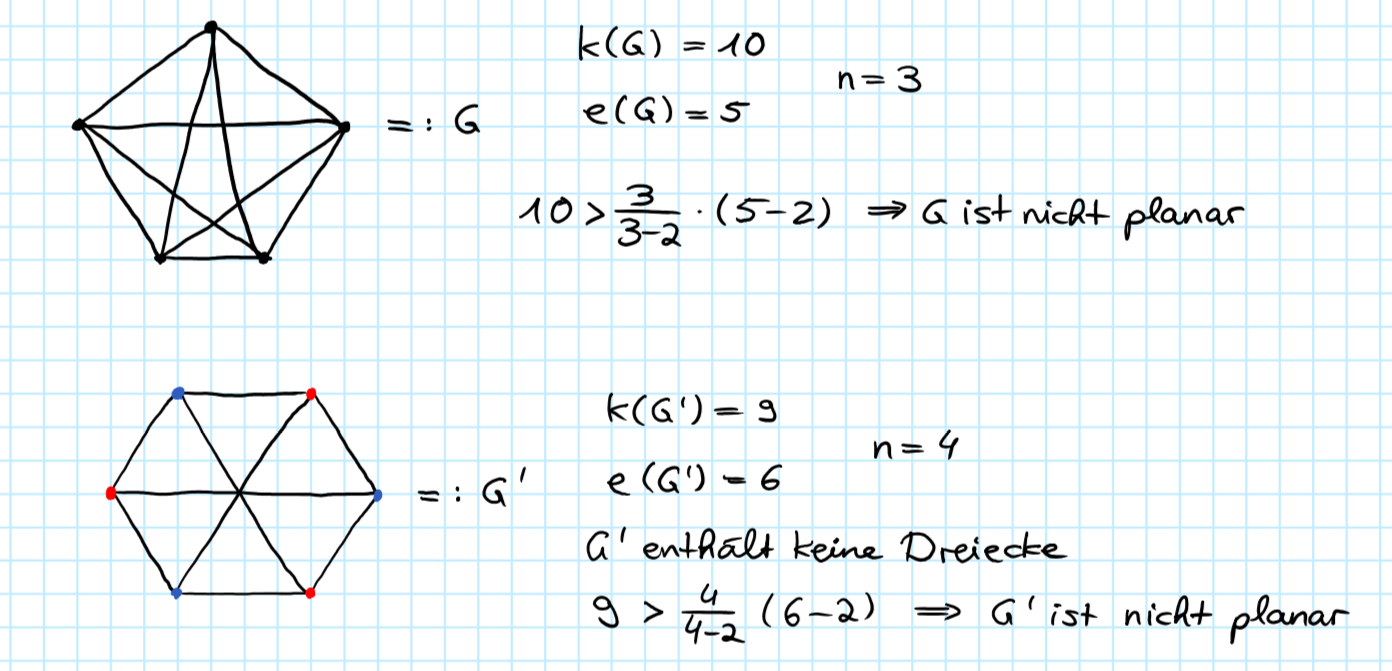
\includegraphics[width=\linewidth]{assets/images/Abb1-15-12.png}
\end{figure}
\end{problem*}

\begin{problem*}[3]

Für einen platonischen Körper $ P \subseteq \mathbb{R}^3 $ mit Zentrum $ 0 $ ist:
\begin{align*}
   Sym(P) &\coloneqq \{ f \in O(3) : f(P) = P \} \\
   Sym_0(P) &\coloneqq \{ f \in SO(3) : f(P) = P \}
 \end{align*} 
Sei $ P $ Würfel.\\
\textbf{Zu zeigen:} 
\begin{itemize}
  \item $Sym(P) = S_4 \times \{ 1, -1 \}$
  \item $Sym_0(P) = S_4$
\end{itemize}
\textbf{Behauptung:} 
$\vert Sym(P) \vert \leq 48, \vert Sym_0(P) \vert \leq 24$.\\
\textbf{Beweis:} Sei $ S $ eine Ecke von $ P $ und seien $ F,G,H $ die zu $ E $ benachbarten Ecken. Da $\phi$ Ecken von $ P $ auf Ecken von $ P $ abbilden, gibt es nur 8 mögliche Werte von $\phi(E)$. Da $ \phi $ benachbarte Ecken auf benachbarte Ecken von $ P $ abbildet, sind $\phi(G), \phi(H), \phi(F)$ in einer von 6 Reihenfolgen die Nachbarn von $ \phi(E) $. Jetzt ist aber $ \phi $ vollständig durch $\phi|_{\{ E,F,G,H \}}$ bestimmt, da $ E,F,G,H $ ein Erzeugendensystem von $\mathbb{R}^3$ ist.\\
Damit ist $ \vert Sym(P) \vert \leq 6 \cdot 8 = 48$. \\
$Sym_0(P) $ ist Untergruppe von $ Sym(P) $. \\
Nach dem Satz von Lagrange ist $\frac{\vert Sym(P) \vert}{\vert Sym_0(P) \vert} \in \mathbb{N} (\star)$.\\
Da $\begin{pmatrix}
	-1 & 0 & 0 \\
	0 & -1 & 0 \\
	0 & 0 & -1 
\end{pmatrix} \in Sym(P)$, aber $det(-I) = (-1)^3 = -1$,\\
ist $I \in Sym(P) \setminus Sym_0(P)$, also ist $\vert Sym(P) \vert > \vert Sym_0(P) \vert $.\\
Wegen $ (\star) $ folgt
\begin{equation*}
	\frac{\vert Sym(P) \vert}{\vert Sym_0(P) \vert} \geq 2 \Rightarrow \vert Sym_0(P) \vert \leq \frac{1}{2} \vert Sym(P) \vert \leq 24.
\end{equation*}
Sei $ D $ die Menge der Hauptdiagonalen von $ P $. Dann ist 
\begin{equation*}
	h: Sym_0(P) \to B_{ ij }(D) \cong S_4, h(\phi) \coloneqq (d \mapsto \phi(d))
\end{equation*}
Gruppenhomomorphismus.\\
% ---------------------------------------------------------------------------------------
% Abbildung einfügen!
%----------------------------------------------------------------------------------------
\textbf{Behauptung:} $ h $ ist surjektiv.\\
Da $ B_{ ij }(D)  $ von Transpositionen erzeugt wird reicht es zu zeigen, dass $ Bild(h) $ jede Transposition enthält. Sei also $ (d_1,d_2) $ eine beliebige Transposition in $ B_{ ij }(D)$.\\
Gesucht: $\phi \in Sym_0(P)$ mit $h(\phi) = (d_1,d_2).$\\
Wähle $ \phi $ als Rotation um $ 180^{ \circ } $ um die gestrichelte Achse (vgl. Abb.), dann ist $\phi(P) = P$, $det(\phi) = 1, \phi(RL) = BL, \phi(BL) = RL, \phi(GL) = GL, \phi(YL) = YL$. Wobei $ GL =$ Grüne Linie, etc.\\ 
Damit ist $h(\phi) = (d_1, d_2).$\\
Wir haben einen surjektiven Hom. $h: Sym_0(P) \to \underset{ \text{Bijektion} }{B_{ij}(D)} $. Aus $ \vert Sym_0(P) \vert \leq 24 = \vert S_4 \vert = \vert B_{ ij }(D) \vert$ folgt sofort, dass $\vert Sym_0(P) \vert = \vert B_{ ij }(D) \vert$ ist und dass $ h $ bijektiv ist:
\begin{equation*}
	Sym_0(P) \cong B_{ ij }(D) \cong S_4.
\end{equation*}
\textbf{Behauptung:} $Sym(P) \cong Sym_0(P) \times \{ -1, 1 \}.$\\
\textbf{Beweis:} Seien:
\begin{align*}
	&g: Sym(P) \to Sym_0(P) \times \{ -1, 1 \}, \psi \mapsto (det(\psi) \cdot \psi,det(\psi)) \\
	&k: Sym_0(P) \times \{ -1, 1 \} \to Sym(P), (\varphi, \varepsilon) \mapsto \varepsilon \phi.
\end{align*}
\textbf{Behauptung:} $ k,g $ sind zueinander Invers.\\
\textbf{Bew:} 
\begin{align*}
	g(k(\varphi,\varepsilon)) &= g(\varepsilon \varphi) = (\varepsilon^3 \cdot \varepsilon \varphi, \varepsilon) = (\varphi, \varepsilon) 
	\\
	k(g(\psi)) &= k(det(\psi) \cdot \psi, det(\psi) ) = det(\psi)^2 \cdot \psi = \psi
\end{align*}
\textbf{Behauptung:} $ k $ ist Hom.\\
\textbf{Beweis:} 
\begin{equation*}
	k((\varphi, \varepsilon)\cdot (\varphi', \varepsilon')) = k(\varphi, \varepsilon) \cdot k(\varphi',\varepsilon').
\end{equation*}
Damit folgt Behauptung. Also ist 
\begin{equation*}
	Sym(P) \cong Sym_0(P) \times \{ -1, 1 \} \cong S_4 \times \{ -1, 1 \}.
\end{equation*}
\end{problem*}

% section 2017_12_15_übungsblatt_8 (end)


\section{2018-01-12 - Übungsblatt 9} % (fold)
\label{sec:2018_01_12_übungsblatt_9}
\textbf{Definition zu Aufgabe 1 (Vgl. Blatt):} Eine trianguliert Fläche $ (M, K, t) $ besteht aus einer Fläche $ M $, einem Simplizialkomplex $ K $ und einem Homöomorphismus $ t: \vert K \vert \to M $.\\
$ (K, t) $ heißt \emph{Triangulierung} von $ M $. \\
Die Eulercharakteristik $ \chi(M) $ ist definiert als $ \chi(K) $, $ \chi(M) $ hängt also nicht von $ (K,t) $ ab.

\begin{problem*}[1]
% ---------------------------------------------------------------------------------------
% vgl. Zeichnung vom Übungsblatt
%----------------------------------------------------------------------------------------
\textbf{Frage:} Ist das eine Triangulierung des Torus $ T $? \\
\textbf{Antwort:} Nein! \\
\textbf{Begründung:} In der Zeichnung werden alle Ecken identifiziert, aber Dreiecke in Simplizialkomplexen haben drei verschiedene Ecken (0-Simplices). Außerdem ist der Schnitt der zwei Dreiecke in er Zeichnung kein Simplex.\\
\\
\textbf{Überlegung:} Was ist dann eine korrekte Triangulierung des Torus $ T $?\\
% ---------------------------------------------------------------------------------------
% Zeichnung einer korrekten Triangulierung mit 32 Dreiecken (4x4 kleine Quadrate)
%----------------------------------------------------------------------------------------
\textbf{Bonusfrage:} Wieviele Dreiecke braucht man mindestens, um einen Torus korrekt zu triangulierung?\\
\textbf{Antwort:} 14! \\
Sei $ (K,t) $ eine Triangulierung des Torus, sei 
\begin{itemize}
    \item $ e$ die Anzahl der Ecken von $ K $.
    \item $ k$ die Anzahl der Kanten von $ K $.
    \item $ s$ die Anzahl der Dreiecke von $ K $.
  \end{itemize}  
Zeichne auf jede Seite von jedem Dreieck "innen" ein Punkt. Sei $ x $ die Anzahl der Punkte.
Da in jedem Dreieck drei Punkte liegen gilt $ x = 3s $. \\
Da in jeder Kante zwei Punkte liegen gilt $ x = 2k $, also $ 3s = 2k $.\\
Der Torus hat Euler-Charakteristik $ 0 $, also gilt
\begin{equation*}
  3 \cdot 0 = 3 \cdot (s - k + e) = 3s - 3k +3e = \underbrace{ (3s -2k) }_{ = 0 } - k + 3e \Rightarrow k = 3e
\end{equation*}
Damit ist $ 2e = \frac{2}{3} k = \frac{2}{3} s = s $. \\
% ---------------------------------------------------------------------------------------
% TODO: Was kann man statt pmatrix verwenden, um eine binom. Koeff. darzustellen? 
%----------------------------------------------------------------------------------------
Da es $\begin{pmatrix}
  e\\
  2  
\end{pmatrix}$
Paare von Ecken gibt und jede Kante ein anderes Eckenpaar als Enden hat, gilt 
$\begin{pmatrix}
  e\\
  2  
\end{pmatrix} \geq k = 3e $
Da $\begin{pmatrix}
  e \\
  2
\end{pmatrix} \geq 3e$ erst ab $ e \geq 7 $ erfüllt ist, gilt $ e \geq 7 $, also $ s = 2e \geq 14 $.\\
Um zu beweisen, dass der kleinste Wert für s genau 14 ist, reicht ein Beispiel: 
%---------------------------------------------------------------------------------------
% Zeichung mit 14 Dreieicken (vgl. Triangulation of Torus)
%----------------------------------------------------------------------------------------
\end{problem*}
\begin{problem*}[2]
\emph{Vorraussetzungen: } Seien $ M_1, M_2 $ zwei Flächen. Für jede Fläche existiert eine triangulierung.\\
\textbf{Behauptung:} $ \chi(M_1 \# M_2) = \chi(M_1) + \chi(M_2) - 2$.\\
\textbf{Lemma 1:} Homöomorphe Flächen haben die gleiche Euler-Charakteristik. \\
\textbf{Beweis:} Sei $\varphi : M \to \tilde{ M }$ Homöo. Sei $ (K,t) $ eine Triangulierung von M. \\
Dann ist $ (K,\varphi \circ t) $ Triangulierung von $ \tilde{ M } $, denn $ \varphi \circ t $ ist Verkettung von Homöomorphismen.\\s
\\
\textbf{Lemma 2:} Seien $ M_1, M_2, N_1, N_2 $ Flächen, sodass $ M_1 \cong N_1, M_2 \cong N_2 $.\\
Dann ist $ M_1 \# M_2 \cong N_1 \# N_2$.\\
\textbf{Beweisansatz:} Seien $ \varphi_1: M_1 \to N_1, \varphi_2: M_2 \to N_2 $ Homöomorphismen.\\
Sei $ M \coloneqq M_1 \# M_2 , N \coloneqq N_1 \# N_2$ beliebige zusammenhängende Summen.\\
Seien $ B_1 \subseteq M_1, B_2 \subseteq M_2 $ die Kreisscheiben, die zur Konstruktion von $ M $ verwendet wurden und sei $ F: \partial B_1 \to \partial B_2$ der verwendete Homöomorphismus.\\
Seien $ C_1 \coloneqq \varphi_1 (B_1), C_2 \coloneqq \varphi_2 (B_2)$. \\
Sei dann $ \tilde{ f } : \partial C_1 \to \partial C_2 $ gegeben durch 
\begin{equation*}
  \tilde{ f }(p) \coloneqq \varphi_2 (f(\varphi_1^{ -1 }(p)))
\end{equation*}
Sei $ \tilde{ N } $ zusammenhängende Summe von $ N_1, N_2 $ mittels $ C_1, C_2, \tilde{ f } $.\\
Dann ist
\begin{equation*}
    \varphi: M \to \tilde{ N }, [p] \mapsto \begin{cases}
    [\varphi_1(p)], $ falls $ p \in M_1 \\
    [\varphi_2(p)], $ falls $ p \in M_2. 
      
    \end{cases}
 \end{equation*}
 ein wohldefinierter Homöomorphismus.\\
 Also ist $M \cong \tilde{ N } \cong N$. \\

\textbf{Beweis der Aufgabe:} \\
Seien $ (K_1, t_1) $ und $(K_2, t_2)$ Triangulierungen von $ M_1 $ und $ M_2 $.\\
Jetzt ist nach \emph{Vorraussetzung} $ M_1 \cong \vert K_1 \vert, M_2 \cong \vert K_2 \vert$ also ist
\begin{equation*}   
M_1 \# M_2 \underset{ \text{ Lemma 2 } }{ \cong } \vert K_1 \vert \# \vert K_2 \vert
 \end{equation*} 
 also auch:
 $$
   \chi (M_1 \# M_2) \underset{ \text{ Lemma 1 } }{ = } (\vert K_1 \vert \# \vert K_2 \vert)
 $$
 wobei wir uns die Verklebung von $ \vert K_1 \vert $ und $\vert K_2 \vert$ beliebig aussuchen dürfen.\\
 Seien also $\triangle_1, \triangle_2$ Dreiecke in $ K_1 $ bzw. $ K_2 $. \\
 Sei $ f: \partial \triangle_1 \to \partial \triangle_2 $ ein Homöomorphismus, der Ecken von $\triangle_1$ auf Ecken von $\triangle_2$ abbildet. \\
 Sei $ S $ die zusammenhängende Summe von $ \vert K_1 \vert $ und $\vert K_2 \vert$ bzgl. 
 $\triangle_1, \triangle_2, f$.\\
 Dann hat $S$ eine durch $ K_1 $ und $ K_2 $ erzeugte simpliziale Struktur.\\
 Es gilt:
 \begin{align*}
   s(K) &= s(K_1) + s(K_2) - 2 \text{ da die Dreiecke fehlen }\\
   k(K) &= k(K_1) + k(K_2) - 3 \text{ da drei Kantenpaare verklebt wurden }\\
   e(K) &= e(K_1) + e(K_2) - 3 \text{ da drei Eckenpaare verklebt wurden}
 \end{align*}
 Also ist 
 $$ \chi(K) = \chi(K_1) + \chi(K_2) - 3 + 3 -2 = \chi(K_1) + \chi(K_2) - 2 $$
 Damit ist 
 \begin{align*}
    \chi(M_1 \# M_2) &= \chi(\vert K_1 \vert \# \vert K_2 \vert) \\
    &= \chi(S) = \chi(K) \\
    &= \chi(K_1) + \chi(K_2) - 2 \\
    &= \chi(M_1) + \chi(M_2) - 2.
  \end{align*} 
\end{problem*}

\begin{problem*}[3]
Sei $ I $ ein Intervall und $c: I \to \mathbb{R}^3 $ eine diff'bare Kurve mit $\frac{dc}{fs}(t) \neq 0$ für alle $ t \in I $.\\
\textbf{Zu zeigen:} Es gibt ein Intervall $ J $ und einen Diffeomorphismus $\varphi : I \to J$, sodass für die umparametrisierte Kurve $ \tilde{ c }: c \circ \varphi^{ -1 } $ die Gleichung 
\begin{equation*}
  \Vert \frac{d\tilde{ c }}{ds}(s) = 1 \Vert
\end{equation*}
für alle $ s \in J $ gilt.\\
\textbf{Beweis:} Sei $ a \in I$ beliebig. Sei $ \varphi: I \to \mathbb{R}$ gegeben durch 
\begin{equation*}
  \varphi(x) \coloneqq \int_a^x { \Vert \frac{dc}{dt}(t) \Vert }dt
\end{equation*}
Da $ \Vert \frac{dc}{dt}(t)  \Vert > 0$ für alle $ t \in I $ ist, ist $ \varphi$ stetig und streng monoton steigend, also ist $ \varphi $ Homöomorphismus von $ I $ nach $ J \coloneqq \varphi (I)$.\\
Nach Konstruktion ist $\varphi$ stetig diff'bar...
\begin{equation*}
  \left( \frac{d \varphi}{dx}(x) = \Vert \frac{dc}{dt}(x) \Vert\right)
\end{equation*}
... mit nicht verschwindender Ableitung also ist $\varphi^{ -1 }$ auch überall stetig diff'bar und damit ist $\varphi$ ein Diffeomorphismus.\\
Sei nun $ \tilde{ c } = c \circ \varphi^{ -1 }$, sei $s_0 \in J$ beliebig. Sei $t_0 = \varphi^{ -1 }(s_0)$\\
Jetzt gilt $c = \tilde{ c } \circ \varphi$, mit Kettenregel folgt:
\begin{align*}
\frac{dc}{dt}(t_0) &= \frac{d \tilde{ c }}{ds}(\varphi(t_0))\cdot \frac{d \varphi}{dt}(t_0) \\
&\Rightarrow \Vert \frac{dc}{dt}(t_0)\Vert = \Vert \frac{d \tilde{ c }}{ds}(s_0) \Vert \cdot \vert \frac{d \varphi}{dt}(t_0) \vert = \Vert \frac{d \tilde{ c }}{ds}(s_0) \Vert \cdot \Vert \frac{dc}{dt}(t_0) \Vert
\end{align*}
Kürzen mit $\Vert \frac{dc}{dt} (t_0) \Vert $
ergibt $ 1 = \Vert \frac{d \tilde{ c }}{ds}(s_0) \Vert $ wie gewünscht.\\

\end{problem*}

% section 2018_01_12_übungsblatt_9 (end)


